\section{THGEM-based sampling elements for DHCAL}
Most recent update: 2020-05-21 \\
Contact person: Shikma Bressler (email: shikma.bressler@cern.ch)
\subsection{Introduction}
Digital Hadronic Calorimetry (DHCAL) for future experiments (e.g. ILC-SiD) requires robust thin sampling elements with high detection efficiency at low pad multiplicity. The large detection area foreseen requires cost-effective solutions.
In recent years, a Weizmann-Aveiro-Coimbra team has shown that sampling elements based on Thick Gaseous Electron Multipliers (THGEM)~\cite{Chechik2004303} could meet DHCAL requirements. The THGEM concept has evolved from a cascade of double-sided electrodes coupled to a pad-anode through an induction gap~\cite{1748-0221-7-05-C05011}, to thinner single-sided WELL detectors - coupled to the pads with and without resistive films~\cite{1748-0221-9-04-P04011,1748-0221-8-07-P07017}.
The most recent and presently leading candidate is the Resistive Plate WELL (RPWELL). It was tested extensively in the laboratory~\cite{1748-0221-8-11-P11004,1748-0221-8-12-C12012} and at muon and high-rate pion beams at CERN-SPS. This very thin single-stage detector yielded a discharge-free operation in different gas mixtures, including Ne- and Ar-based ones, providing high detection efficiency at low pad multiplicity.

\subsubsection{The Resistive Plate WELL}
The Resistive Plate WELL (RPWELL) is a single-sided THGEM (with copper clad on one side only), coupled to the readout pads through a material sheet with high bulk resistivity (see Figure~\ref{fig:Calorimeter:THGEM:rpwell}). Materials with bulk resistivity in the $\SI{e9}{\ohm cm}$ scale prevent significant drops of gain, and hence efficiency, at high particle flux~\cite{1748-0221-8-11-P11004}.
\begin{figure}
	\centering
	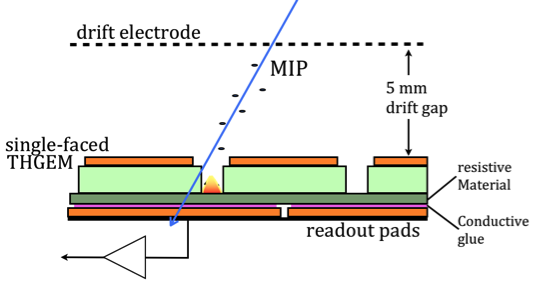
\includegraphics[width=.5\textwidth]{Calorimeter/THGEM/rpwell.png}
	\caption{The RPWELL configuration with a resistive anode and a readout electrode. The WELL, a single-faced THGEM, is coupled to a readout anode (e.g. with strips or pads) via a resistive plate.}
	\label{fig:Calorimeter:THGEM:rpwell}
\end{figure}
\subsection{Recent Milestones with Small and Medium Size RPWELL Prototypes}
Small ($10\times \SI{10}{cm^2}$) and medium size ($30\times \SI{30}{cm^2}$) RPWELL detector prototypes were built and tested in the laboratory and at the CERN-SPS. The \SI{0.8}{mm} thick WELL electrodes were coupled to $1\times \SI{1}{cm^2}$ copper pads through \SI{0.4}{mm} thick Semitron ESD225 resistive polymer ($\approx \SI{e9}{\ohm cm}$ bulk resistivity). With a \SI{5}{mm} drift gap the sampling element had a total thickness of \SI{6.2}{mm} (excluding readout electronics -- here SRS-APV~\cite{1748-0221-8-03-C03015,French2001359}).
The detection efficiency as a function of pad multiplicity (with low rate muons) is shown for the two prototypes in Figure~\ref{fig:Calorimeter:THGEM:efficiencyVSMultiplicity}. Both detectors reached high detection efficiency at low pad multiplicity when operated in our traditional Ne/5\%\ce{CH4} (Figure~\ref{fig:Calorimeter:THGEM:efficiencyVSMultiplicity} left; operation voltage, V, in the range $\SIrange{800}{930}{V}$) and in the cost-effective Ar/5\%\ce{CH4} (Figure~\ref{fig:Calorimeter:THGEM:efficiencyVSMultiplicity} right; V in the range $\SIrange{1500}{1720}{V}$) gas mixtures.
\begin{figure}
	\centering
	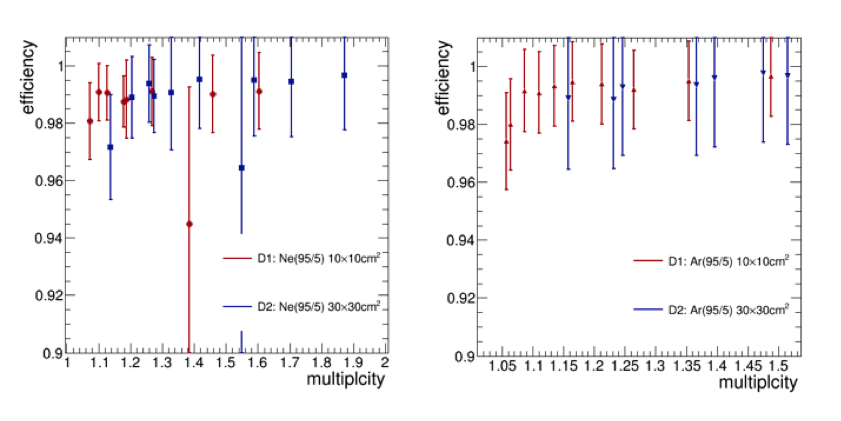
\includegraphics[width=.9\textwidth]{Calorimeter/THGEM/efficiencyVSMultiplicity.png}
	\caption{Efficiency as a function of the average pad multiplicity measured with the $10\times \SI{10}{cm^2}$ and $30\times \SI{30}{cm^2}$ detectors in muon beam. Left: Ne/5\%\ce{CH4} gas mixture. Right: Ar/5\%\ce{CH4} gas mixture}
	\label{fig:Calorimeter:THGEM:efficiencyVSMultiplicity}
\end{figure}
\begin{figure}
	\centering
	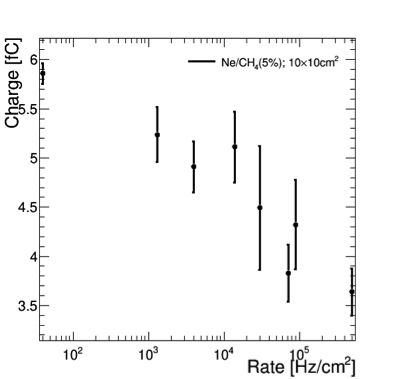
\includegraphics[width=.5\textwidth]{Calorimeter/THGEM/charge_vs_rate.png}
	\caption{The charge (estimated from the spectra most probable value) as a function of the incoming particle flux.  All the measurements were conducted at Ne/5\%\ce{CH4} gas mixture at the same operation voltage of \SI{880}{V}. A pion beam was used to generate the high incoming fluxes.}
	\label{fig:Calorimeter:THGEM:chargeVsRate}
\end{figure}
Figure~\ref{fig:Calorimeter:THGEM:chargeVsRate} shows the measured gain as a function of the particle flux; the same operation voltage of \SI{880}{V} was maintained throughout the measurements (with low rate muons as well as high rate pions). A moderate gain-drop of $\approx 30\%$ was measured while the flux was increased by 3 orders of magnitude (from 50 to $\SI{e5}{Hz/cm^2}$). It resulted in a negligible efficiency drop, since the pulse-over-threshold was sufficiently high.
Most importantly, during the two weeks of in-beam operation (which included also long time operation under high rate, $\SI{e5}{Hz/cm^2}$, pion beam), with both Ne-based and Ar-based gas mixtures, the small prototype was completely discharge-free. The resulting discharge probability is therefore below $10^{-8}$. Occasional discharges occurring in the medium-size prototypes were traced to be associated with defects in some support pins within the active area; these were avoided in the next prototypes.
The RPWELL laboratory and test-beam results with the $\SI{10}\times\SI{10}{cm^2}$ and $\SI{30}\times\SI{30}{cm^2}$ detector prototypes are summarized in \cite{Moleri:2016hgk,Moleri:2016bjv}.

\subsubsection{Preliminary performance of $\SI{50}\times\SI{50}{cm^2}$ RPWELL prototypes}

Having in mind their application to (S)DHCAL, techniques were developed for producing large-area ($\SI{48} \times \SI{48}{cm^2}$) \SI{4.5}{mm} thick (excluding electronics) detectors, incorporating \SI{e10}{\ohm\centi\meter} silicate glass resistive plates (Figure~\ref{fig:Calorimeter:THGEM:glueing}). Five such detectors were built and equipped with a pad-anode embedding ILC-(S)DHCAL MICROROC chips~\cite{Adloff_2012} and has a total thickness of \SI{6.5}{mm}. The RPWELL differed by their electrode quality, of which the thickness variation ranged from 5\% (best) to 25\% (worst), affecting significantly their stability and hence performance.
\begin{figure}
	\centering
	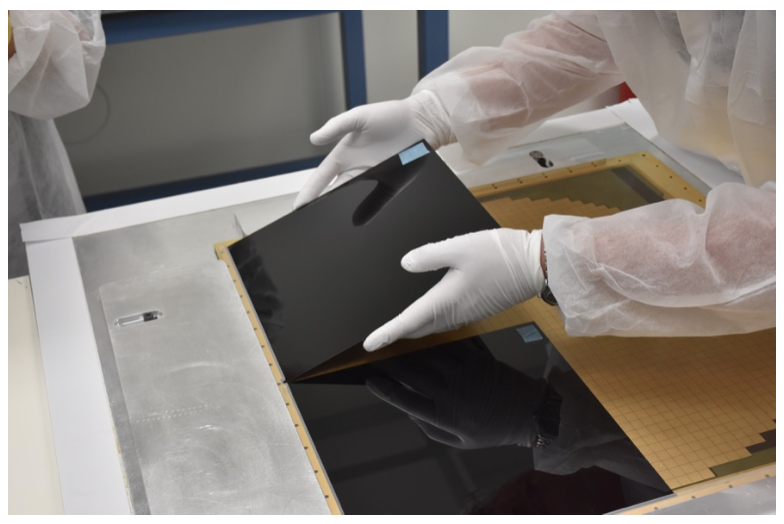
\includegraphics[width=.5\textwidth]{Calorimeter/THGEM/resistivePlateGlueing}
	\caption{The gluing of the glass resistive plate to the pad-anode. Part of the assembly procedure.}
	\label{fig:Calorimeter:THGEM:glueing}
\end{figure}

During August 2018, the first SDHCAL sampling element prototype built (with 25\% thickness variation) has been investigated at CERN/SPS, in Ar/(7\%)CO2, with muons and high-rate pions. Preliminary analysis results confirm that the performance of this prototype would be suitable for (S)DHCAL; $\geq 95\%$ detection efficiency across most of the surface was achieved with a pad multiplicity of $\approx 1$ in most events (average value of 1.7 due to a small number of events with tens of pads firing - probably indicating a discharge). Some efficiency variations are attributed to the large electrode-thickness variations (thus gain). The result obtained with these prototypes as well as those obtained with a small (S)DHCAL comprising several MICROMEGAS, and several RPWELL-based sampling elements are summarized in~\cite{Bressler:2019uyt}.

\subsection{Engineering Challenges}
%The novel design of a large RPWELL detector prototype (without the present support pins) is completed. Assembly and tests are foreseen in the coming year. Upon success, we are confident that future chambers could be fully industrially produced. We are currently investigating, with industry, alternative materials and production technologies of THGEM electrodes; similarly, we are considering different resistive-plate materials, with of appropriate bulk resistivity.

\subsection{Future Plans}
The experience gained with the $\SI{50} \times \SI{50}{cm^2}$ RPWELL prototypes emphasizes the need to use electrodes with much smaller thickness variations, probably below 5\%. It also points towards the need to improve the assembly technique, and in particular ensure that no glue penetrates into the holes. New gluing techniques will be tested in the coming future and the new assembled prototypes will be tested in the laboratory and in muon and pion beams. 
Once suitable sampling elements are built, we foresee additional test beam campaign of an RPWELL or MOGD base (S)DHCAL prototype. 
